\documentclass[a4paper,12pt]{article}

\usepackage{graphicx}
\usepackage{geometry}
\usepackage{lipsum} % For generating dummy text
\usepackage{svg}

\geometry{margin=1in}

\begin{document}

\begin{figure}[h]
	\centering
	\includesvg[width=3in]{images/logo-white.svg}
	\caption{Logo}
\end{figure}
\title{Go2Me}
\author{Rui Esteves Araújo\\Faculdade de Engenharia       
\maketitle

\section*{Introduction}
This section provides an introduction to the car platooning project.

\section{Date: 2024-01-16}
\subsection{Overview}
Today, I conducted research on existing car platooning technologies and reviewed relevant literature.

\subsection{Key Findings}
\begin{itemize}
    \item Car platooning improves fuel efficiency by maintaining close vehicle spacing.
    \item Various communication protocols are used for inter-vehicle communication.
\end{itemize}

\section{Date: 2024-01-17}
\subsection{Experiment Setup}
\lipsum[1-2] % Placeholder for experimental details

\subsection{Results}
\begin{figure}[h]
    \centering
    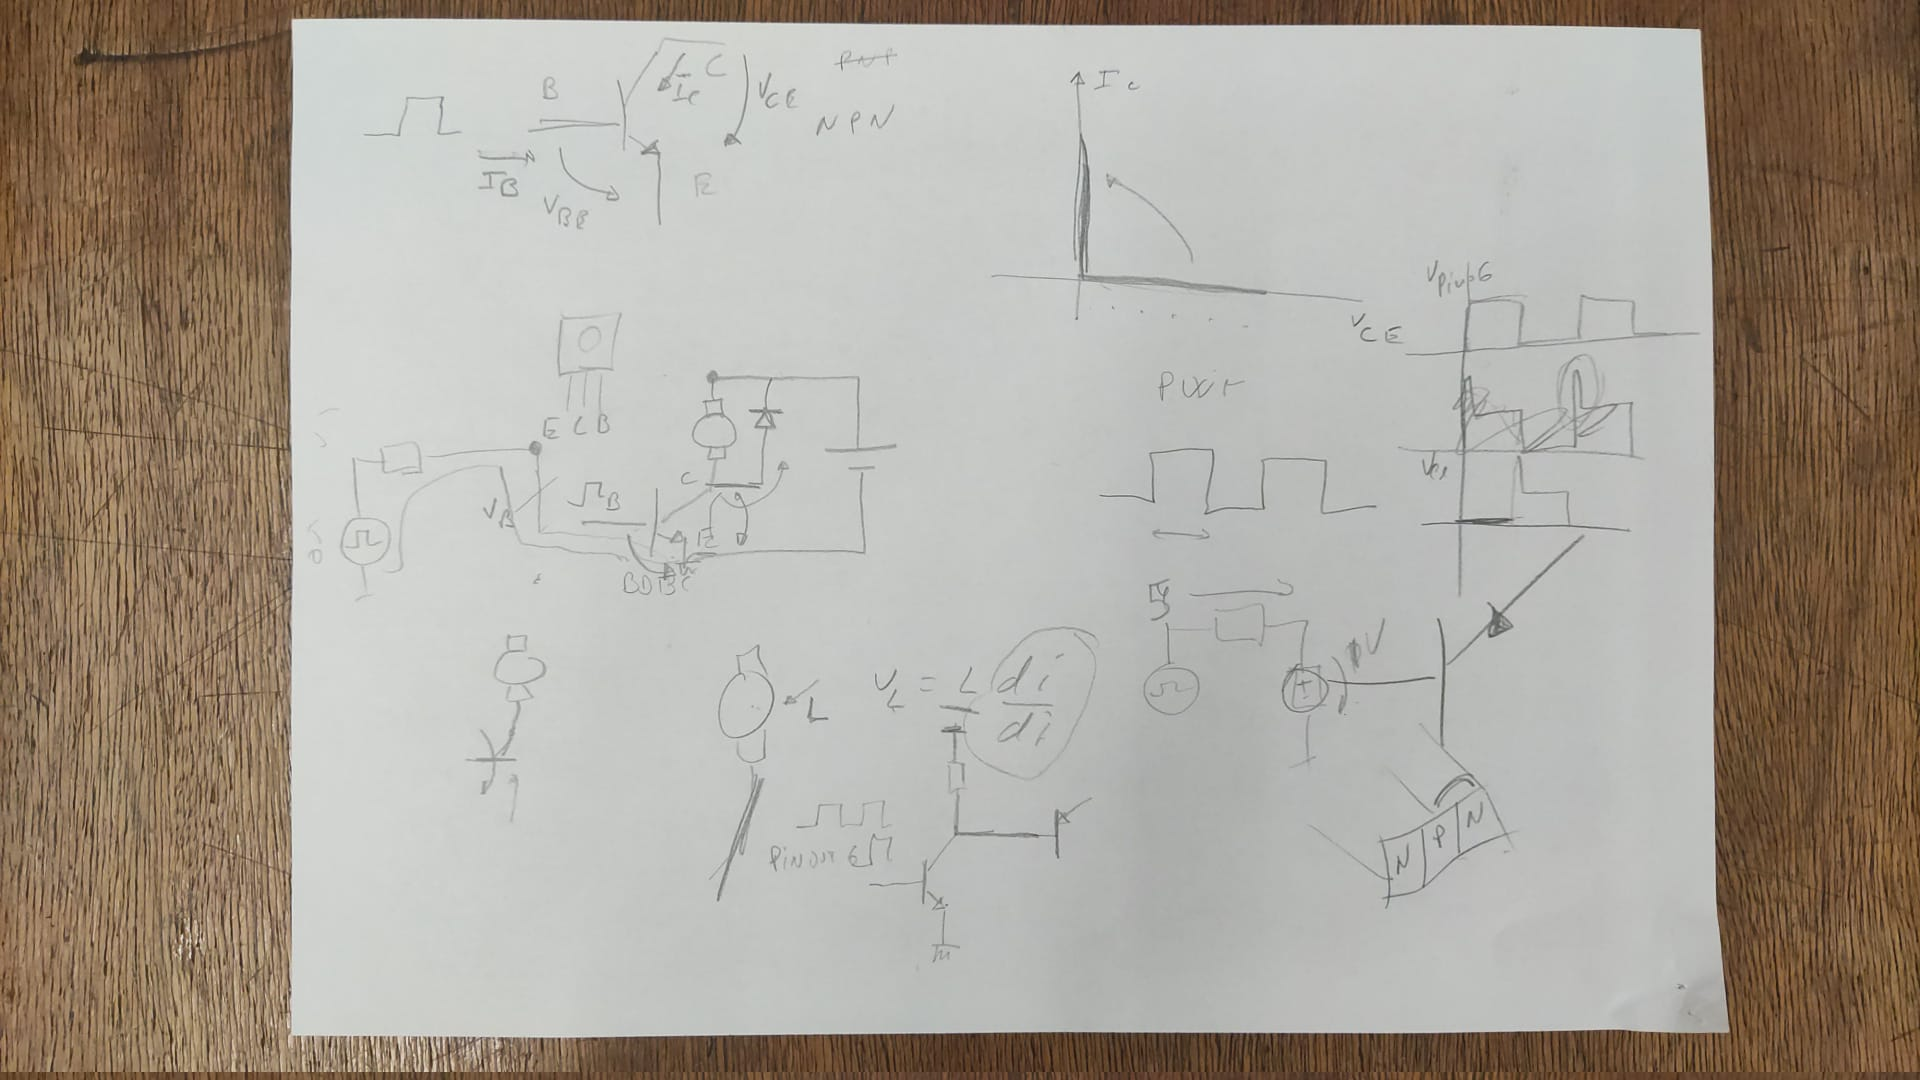
\includegraphics[width=0.8\textwidth, natwidth=1920, natheight=1080]{images/motor-circuit_16-01-2024.jpeg}
    \caption{Experimental Setup Diagram}
    \label{fig:experiment_diagram}
\end{figure}

\lipsum[3] % Placeholder for experimental results

\section*{Conclusion}
Summarize key findings and outline next steps.

\end{document}
